\section{Geometric Control and Mechanics}

\begin{frame}
	\frametitle{Geometric Mechanics}
	
	\begin{itemize}
		\item Introduced by:
		\begin{itemize}
			\item F. Bullo and A. Lewis, 2005. \footcite{bulloBook}
			\item T. Lee, 2008. \footcite{Lee2008ComputationalGM}
			%\footcite{Taeyoung Lee, Computational geometric mechanics and control of rigid bodies}
			\item T. Lee et al. 2018. \footcite{LeeModel} 
		\end{itemize}
	
	\end{itemize}
	\begin{itemize}
		\item Rotating rigid body dynamics equation:
	\end{itemize}	
	\begin{equation}
		m \ddot{\textbf{x}} + m g\textbf{e}_3 = f\text{R}\textbf{e}_3 \label{model1}
	\end{equation}
	\begin{equation}
		\text{J}\dot{\mb{\Omega}} + \mb{\Omega} \times \text{J}\mb{\Omega} = \textbf{M} \label{model2}
	\end{equation}
	\begin{equation}                       
		\dot{\text{R}} = \text{R}\widehat{\mb{\Omega}} \label{model3}
	\end{equation}
	
\end{frame}

\begin{frame}
	\frametitle{Geometric Control (1)}

	\begin{itemize}
		\item PD control with nonlinear terms
		\item First developed by T. Lee et al. 2010. \footcite{LeeClanak4}
		\item  T. Lee et al. 2011. \footcite{LeeClanak3} - Robust geometric control
		\item Kotaru et al. 2019. \footcite{Kotaru2019GeometricLA} - L1 Aadaptive controller
		\item  S. Lee et al. 2019. \footcite{Lee2019} - Parameter tuning optimization
	\end{itemize}
\end{frame}

\begin{frame}
	\frametitle{Geometric Control (2) \footcite{Markovic2019}}
	
	\begin{columns}
		\begin{column}{0.5\textwidth}\centering
			\begin{figure}[H]
				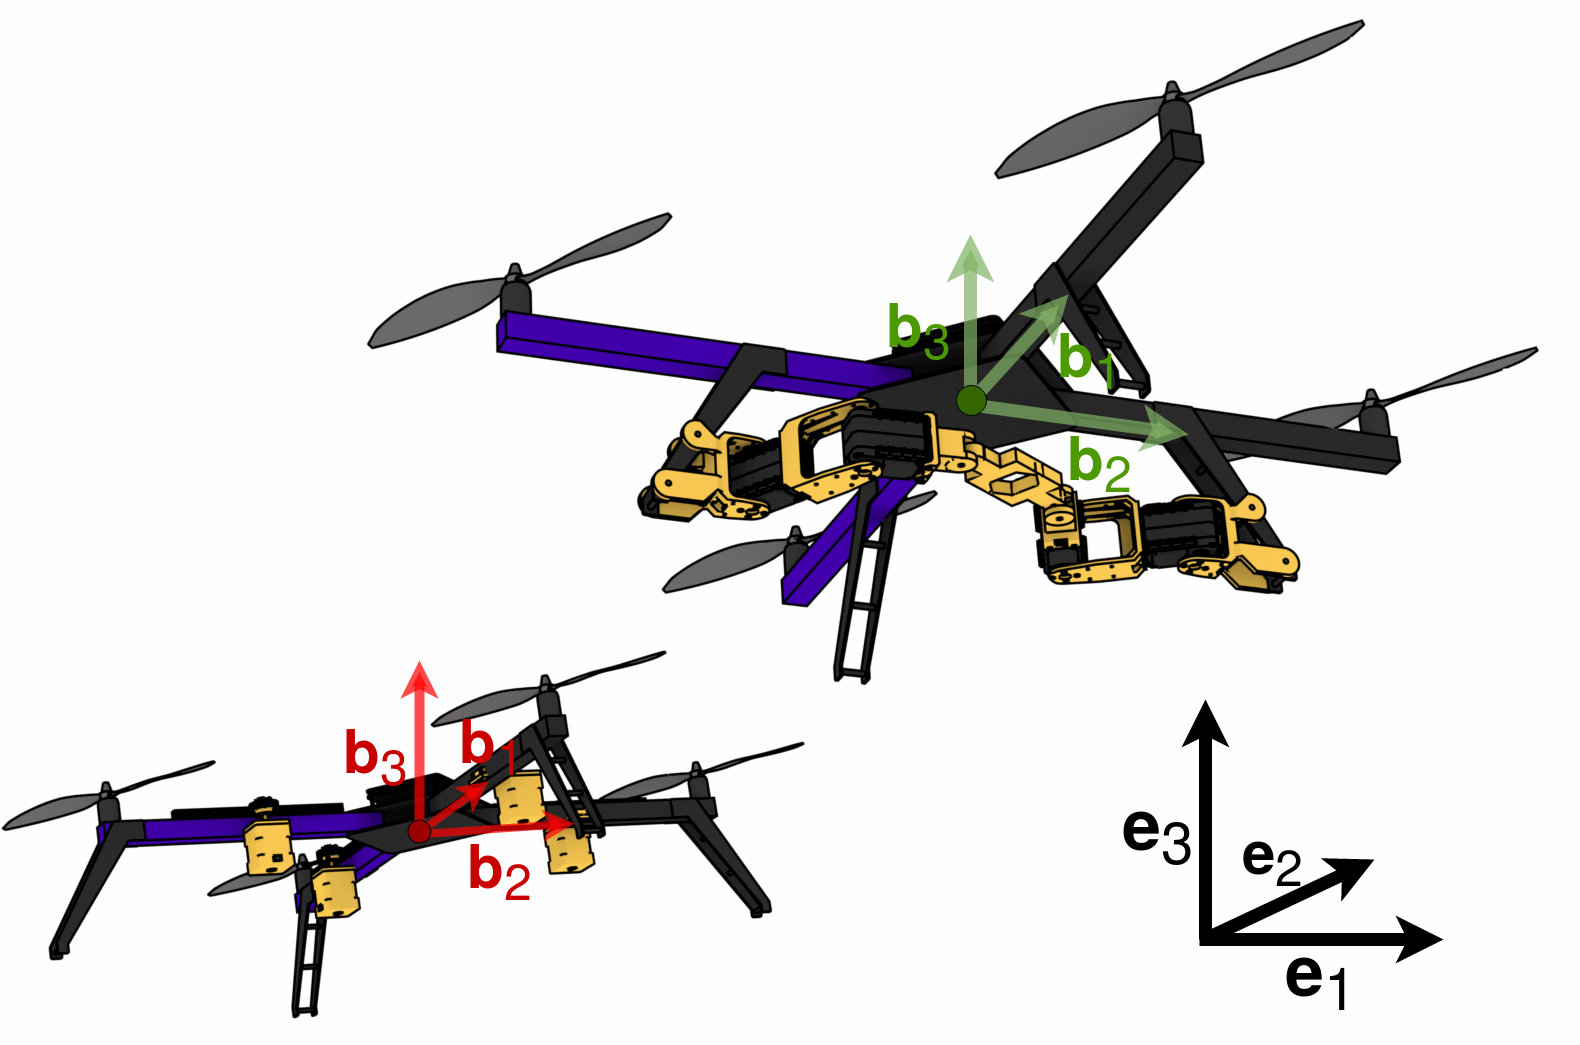
\includegraphics[width=0.8\columnwidth]{figures/uav.png}	
				\centering
				\caption{Two UAVs endowed with variable center of gravity by moving masses and manipulator carried payload (top). Position tracking results (right)${}^{8}$. }
				\label{fig:uav_model}
			\end{figure}
		\end{column}
		
		\begin{column}{0.5\textwidth}\centering
			\begin{figure}
				\centering
				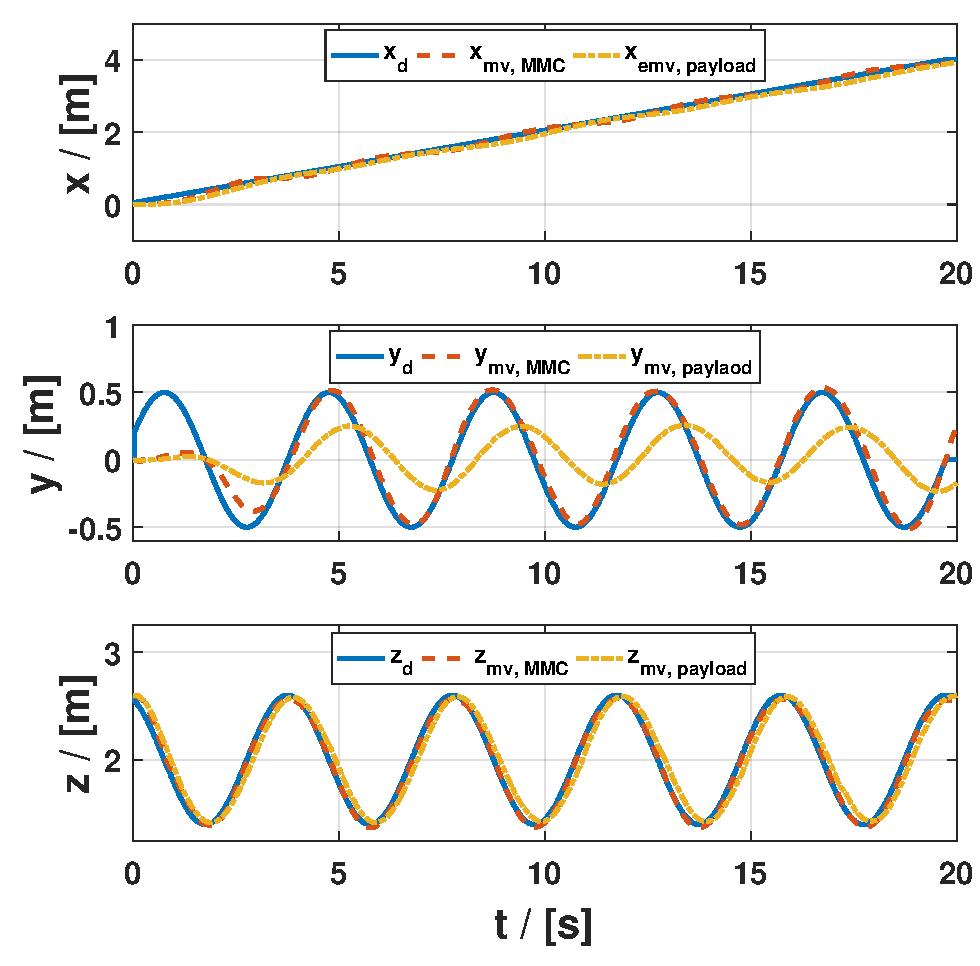
\includegraphics[width=0.95\columnwidth]{figures/both_pos_crop.pdf}
				\label{fig:traj_pos}
			\end{figure}
		\end{column}
	\end{columns}
\end{frame}

\begin{frame}
	\frametitle{Gemetric Control - Transportation Tasks (1)}
	
	\begin{itemize}
		\item Introduced by T. Lee and V. Kumar 2013. \footcite{cable-load1}
		\item A. Goodarzi and T. Lee 2015. \footcite{cable-load-multiple} - Multiple quadrotors employed
		\item  A. Goodarzi and T. Lee 2015. \footcite{flexible-cable-dynamics} and A. Goodarzi et al. 2013. \footcite{stabilization-flexible-cable} - Adaptive control with unknown mass variations
	\end{itemize}
\end{frame}

\begin{frame}
	\frametitle{Geometric Control - Transportation Tasks (2) \footcite{Lee2014GeometricCO}}
	
	\begin{columns}
		\begin{column}{0.5\textwidth}\centering
			\begin{itemize}
				\item Multiple quadrotor UAVs carrying a rigid body payload via cables
				\item Cable configuration lies in $\text{S}^2$ - spherical Lie group
				\item Complete system configuration lies in $\text{SE(3)} \times \text{S}^2$
				\item Payload position and attitude tracking problem
			\end{itemize}
		\end{column}
		
		\begin{column}{0.5\textwidth}\centering
			\begin{figure}[H]
				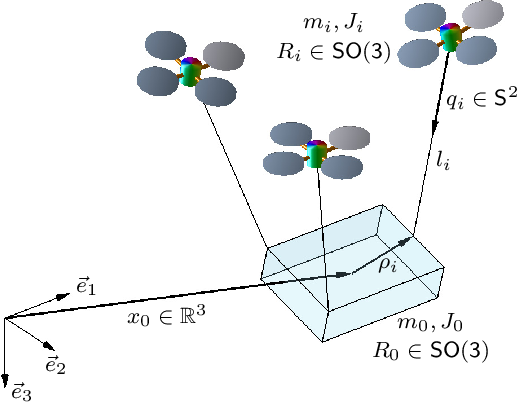
\includegraphics[width=0.9\columnwidth]{figures/payload_carrying.png}
				\caption{Payload transportation with multiple UAVs${}^{13}$}
				\centering
			\end{figure}
		\end{column}
	\end{columns}
		
\end{frame}